\documentclass[tikz,border=12pt]{standalone}
\usepackage[T1]{fontenc}
\usepackage{tgheros}
\usepackage{sfmath}
\usepackage{amsmath}
% % \usepackage{fontawesome5} (Removed for publication-grade academic typography) (Removed for publication-grade academic typography)
\usepackage{tikz}
\usetikzlibrary{arrows.meta,positioning,shapes.geometric,fit,backgrounds,calc}
\usepackage{xcolor}

\renewcommand{\familydefault}{\sfdefault}

% Harvard Crimson & ETH Zurich Academic Semantic Palette
\definecolor{harvardcrimson}{HTML}{A51C30}
\definecolor{ethdarkblue}{HTML}{1F407A}
\definecolor{ethblue}{HTML}{215CAF}
\definecolor{ethpetrol}{HTML}{007A87}
\definecolor{ethbronze}{HTML}{B87333}
\definecolor{ethpurple}{HTML}{5B4B8A}
\definecolor{ethslate}{HTML}{475569}
\definecolor{cardbg}{HTML}{F8FAFC}
\definecolor{cardborder}{HTML}{CBD5E1}
\definecolor{safeTeal}{HTML}{10B981}

\begin{document}
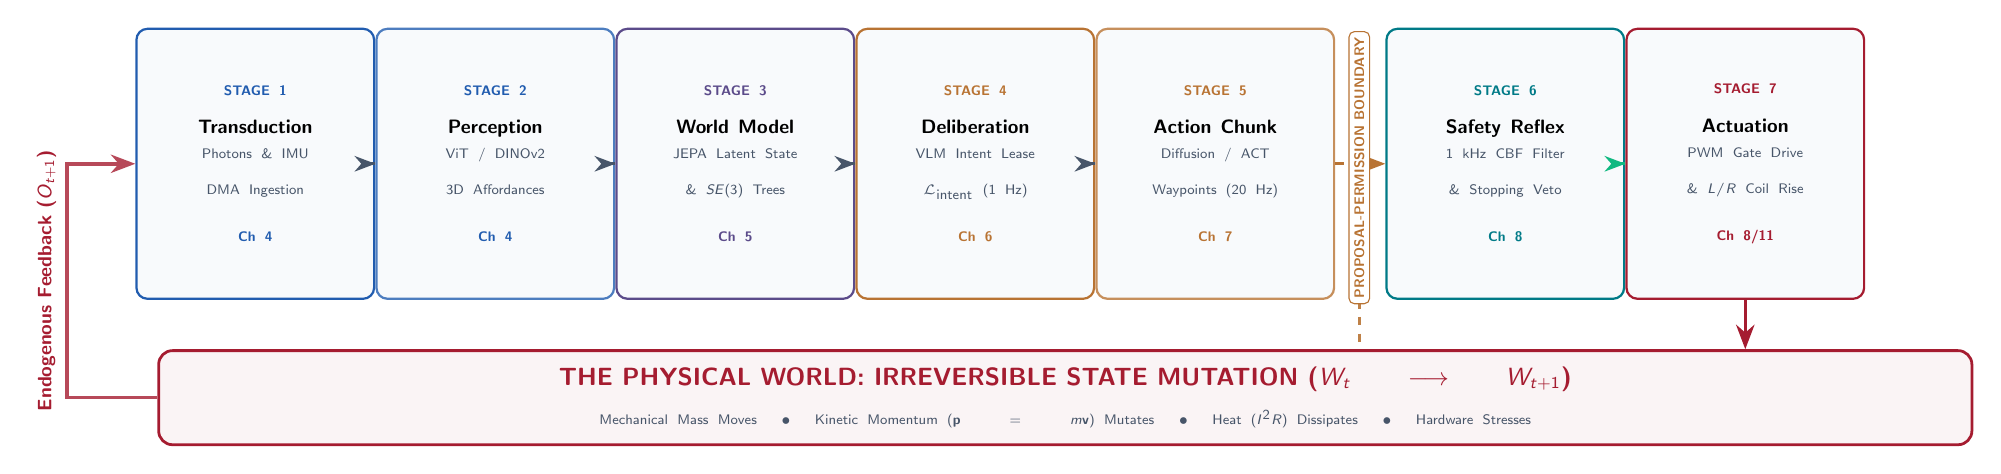
\begin{tikzpicture}[
  font=\sffamily,
  >=Stealth,
  flowbox/.style={
    draw=cardborder,
    fill=cardbg,
    rounded corners=4pt,
    line width=0.8pt,
    text width=1.05in,
    minimum height=1.35in,
    inner sep=5pt,
    align=center,
    anchor=north
  }
]

  % Top Title Banner
  % (Top title banner removed for academic publication standards)
% ROW 1: SENSING, PERCEPTION & STATE
  \node[flowbox, draw=ethblue] (b1) at (0.40in, 0.00in) {
    {\tiny\bfseries\color{ethblue} STAGE 1}\\[2pt]
    {\scriptsize\bfseries Transduction}\\[3pt]
    {\tiny\color{ethslate}Photons \& IMU\\[1pt]DMA Ingestion}\\[5pt]
    {\tiny\textbf{\color{ethblue}Ch 4}}
  };

  \node[flowbox, draw=ethblue!80] (b2) at (1.60in, 0.00in) {
    {\tiny\bfseries\color{ethblue} STAGE 2}\\[2pt]
    {\scriptsize\bfseries Perception}\\[3pt]
    {\tiny\color{ethslate}ViT / DINOv2\\[1pt]3D Affordances}\\[5pt]
    {\tiny\textbf{\color{ethblue}Ch 4}}
  };

  \node[flowbox, draw=ethpurple] (b3) at (2.80in, 0.00in) {
    {\tiny\bfseries\color{ethpurple} STAGE 3}\\[2pt]
    {\scriptsize\bfseries World Model}\\[3pt]
    {\tiny\color{ethslate}JEPA Latent State\\[1pt]\& $SE(3)$ Trees}\\[5pt]
    {\tiny\textbf{\color{ethpurple}Ch 5}}
  };

  \node[flowbox, draw=ethbronze] (b4) at (4.00in, 0.00in) {
    {\tiny\bfseries\color{ethbronze} STAGE 4}\\[2pt]
    {\scriptsize\bfseries Deliberation}\\[3pt]
    {\tiny\color{ethslate}VLM Intent Lease\\[1pt]$\mathcal{L}_{\text{intent}}$ ($1\text{ Hz}$)}\\[5pt]
    {\tiny\textbf{\color{ethbronze}Ch 6}}
  };

  \node[flowbox, draw=ethbronze!80] (b5) at (5.20in, 0.00in) {
    {\tiny\bfseries\color{ethbronze} STAGE 5}\\[2pt]
    {\scriptsize\bfseries Action Chunk}\\[3pt]
    {\tiny\color{ethslate}Diffusion / ACT\\[1pt]Waypoints ($20\text{ Hz}$)}\\[5pt]
    {\tiny\textbf{\color{ethbronze}Ch 7}}
  };

  \node[flowbox, draw=ethpetrol] (b6) at (6.65in, 0.00in) {
    {\tiny\bfseries\color{ethpetrol} STAGE 6}\\[2pt]
    {\scriptsize\bfseries Safety Reflex}\\[3pt]
    {\tiny\color{ethslate}1 kHz CBF Filter\\[1pt]\& Stopping Veto}\\[5pt]
    {\tiny\textbf{\color{ethpetrol}Ch 8}}
  };

  \node[flowbox, draw=harvardcrimson] (b7) at (7.85in, 0.00in) {
    {\tiny\bfseries\color{harvardcrimson} STAGE 7}\\[2pt]
    {\scriptsize\bfseries Actuation}\\[3pt]
    {\tiny\color{ethslate}PWM Gate Drive\\[1pt]\& $L/R$ Coil Rise}\\[5pt]
    {\tiny\textbf{\color{harvardcrimson}Ch 8/11}}
  };

  % Dataflow Arrows Across Top Row
  \draw[->, line width=1pt, draw=ethslate] (b1.east) -- (b2.west);
  \draw[->, line width=1pt, draw=ethslate] (b2.east) -- (b3.west);
  \draw[->, line width=1pt, draw=ethslate] (b3.east) -- (b4.west);
  \draw[->, line width=1pt, draw=ethslate] (b4.east) -- (b5.west);
  \draw[->, line width=1pt, dashed, draw=ethbronze] (b5.east) -- (b6.west);
  \draw[->, line width=1pt, draw=safeTeal] (b6.east) -- (b7.west);

  % Proposal-Permission Boundary Divider Line
  \draw[dashed, line width=1.2pt, draw=ethbronze!90] (5.92in, -0.45in) -- (5.92in, -2.05in);
  \node[font=\sffamily\bfseries\tiny, fill=white, draw=ethbronze, rounded corners=2pt, inner sep=2pt, text=ethbronze, rotate=90] at (5.92in, -0.70in) {PROPOSAL-PERMISSION BOUNDARY};

  % Bottom Physical World Box ($W_t \to W_{t+1}$)
  \node[draw=harvardcrimson, fill=harvardcrimson!5, rounded corners=5pt, line width=1pt, text width=8.90in, inner sep=6pt, align=center] (world) at (4.45in, -1.85in) {
    {\small\bfseries\color{harvardcrimson} THE PHYSICAL WORLD: IRREVERSIBLE STATE MUTATION ($W_t \longrightarrow W_{t+1}$)}\\[2pt]
    {\tiny\color{ethslate}Mechanical Mass Moves $\quad\bullet\quad$ Kinetic Momentum ($\mathbf{p} = m\mathbf{v}$) Mutates $\quad\bullet\quad$ Heat ($I^2R$) Dissipates $\quad\bullet\quad$ Hardware Stresses}
  };

  % Actuation to World Arrow
  \draw[->, line width=1.3pt, draw=harvardcrimson] (b7.south) -- (b7.south |- world.north);

  % Endogenous Feedback Loop from World back to Stage 1 (Wide loop with 0.45in clearance)
  \draw[->, line width=1.3pt, draw=harvardcrimson!80] (world.west) -- ++(-0.45in, 0) |- (b1.west)
    node[pos=0.25, above, rotate=90, font=\sffamily\bfseries\scriptsize, text=harvardcrimson] { Endogenous Feedback ($O_{t+1}$)};

\end{tikzpicture}
\end{document}
